\documentclass[../2.tex]{subfiles}
\begin{document}

    An relevant differential equation in physics and mathematics is the so called \ii{heat equation}
    \[ \frac{df}{dt} = -\Delta f . \]
    % \begin{prop}
    %     Let $\ch{\rho} \in C_0$ be a time dependent chain on our graph representing a density, and let the mass $M = \sum_{\ch{i}\in C_0} \braket{i}{\rho}$ be 
    %     a conserved quantity, then given a flux for $\ch{\rho}$, namely a time dependent $\ch{j} \in C_1$ such that
    %     $\ch{j} = \del_1^\dagger \ch{\rho}$, then $\ch{\rho}$ satisfies the discrete heat equation
    %     \[ \frac{\del}{\del t} \ch{\rho} = -\Delta_0 \ch{\rho}. \]
    % \end{prop}
    % \begin{proof}
    %     Since the mass $M$ is a conserved quantity, we need the flux on the coboundary of any vertex set $A$ added to the variation of 
    %     the mass within $A$ to be zero, hence a local continuity equation.
    %     The vertex set $A$ can be seen as the chain $\ch{A} = \sum_{i \in A}\ch{i}$, with this notation we have that
    %     the previous sentece reads as
    %     \[ \frac{d}{dt}\braket{A}{\rho} + \cc{A}\del_1\ch{j} = 0 . \]
    %     In fact, $\cc{A}\del_1\ch{j}=\cc{j}\del_1^\dagger\ch{A}$ is the flux evaluated on the coboundary of $A$ $\del_1^\dagger\ch{A}$.\\
    %     It follows that 
    %     \[ \frac{d}{dt}\braket{A}{\rho} + \cc{A}\del_1\ch{j} = \sum_{i \in A}\cc{i}(\frac{d}{dt}\ch{\rho}+\del_1\ch{j}) = 0, \]
    %     since $\cc{i}$ is not time dependent, which leads to the local continuity equation 
    %     \[ \frac{d}{dt}\ch{\rho}+\del_1\ch{j} = 0. \]
    %     Inserting the definition of flux in the continuity equation we obtain the discrete heat equation on graphs
    %     \[ \frac{d}{dt}\ch{\rho}+\del_1\del_1^\dagger \ch{\rho} = \frac{d}{dt}\ch{\rho}+\Delta_0 \ch{\rho} = 0.\]\qedhere    
    % \end{proof}
    
    % We can therefore interpret the heat equation on graphs as a counter-gradient diffusion of some conserved quantity.
    Let us see what we can say about the solution of this equation on graphs.

    \begin{prop}
        Let $\frac{d}{dt}\ch{\psi} = -\Delta_0 \ch{\psi}$ and $\ch{\psi}|_{t = 0} = \ch{\psi_0}$, then
        \[ \ch{\psi} = \sum_i\ch{e_i}e^{-\lambda_i t}\braket{e_i}{\psi_0}, \]
        where $\ch{e_i}$ and $\lambda_i$ are the orthonornmal eigenchains and the eigenvalues of the $0$-laplacian respectively,
        i.e. $\Delta_0\ch{e_i} =\ch{e_i}\lambda_i$.
    \end{prop}
    \begin{proof}
        Since $\Delta_0$ is selfadjoint and therefore admits the expansion $\Delta_0 = \sum_i \ch{e_i}\lambda_i\cc{e_i}$,
        where $\ch{e_i}$ and $\lambda_i$ are the orthonornmal eigenchains and the eigenvalues of the $0$-laplacian respectively,
        i.e. $\Delta_0\ch{e_i} =\ch{e_i}\lambda_i$. The discrete heat equation is linear and with constant coefficients and therefore
        it admits a solution of the type $\ch{\psi} = e^{-\Delta_0 t}\ch{\psi_0}$.
        Since $[\Delta_0, e^{-\Delta_0 t}] = 0$, these two operators share the eigenchains and therefore we also have that
        \[ e^{-\Delta_0 t} = \sum_i \ch{e_i}e^{-\lambda_i t} \cc{e_i},\]
        hence the solution. \qedhere
    \end{proof}

    From this solution we can notice that for $t \to \infty$, the only terms left are those with eigenvalue $0$, namely the connected components.
    However, because of the term $\braket{e_i}{\psi_0}$, only the connected components on which $\ch{\psi_0}$ is not zero everywhere remain.

    \begin{figure}[H]
        \centering
        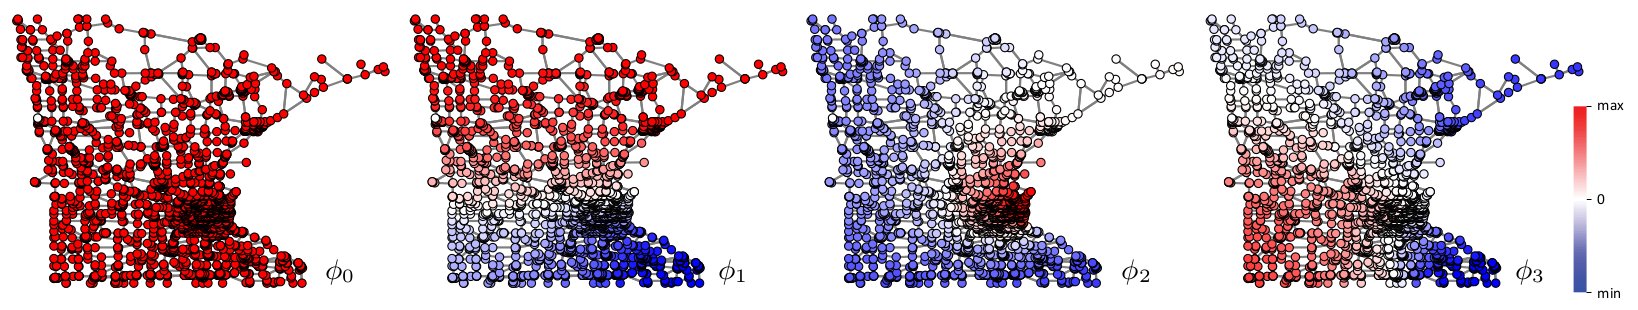
\includegraphics[width=17cm, height=4cm]{sections/2/eiglap}
        \caption{A graphical representation of the first laplacian eigenchains.}
        \label{fig:2:5}
    \end{figure}

    \begin{exa}
        Let's for instance take the graph in Fig. \ref{fig:2:3}. On this graph we want to solve the heat equation given the initial condition
        $\ch{\psi_0} = \ch{2}+\ch{8}$. Since the subgroup generated by $\{\ch{4},\ch{5},\ch{6},\ch{7}\}$ has a null projection on the initial condition, being an 
        invariant subgroup under $\Delta_0$ and $e^{-\Delta_0 t}$, we have that those vertices do not appear in the final solution.
        In order to write the solution we need to diagonalize the other two blocks of the $0$-laplacian.
        For the block of $\{\ch{1},\ch{2},\ch{3}\}$, we have 
        \[ \Delta_0 \frac{\ch{1}+\ch{2}+\ch{3}}{\sqrt{3}} = 0 , \;
        \Delta_0 \frac{\ch{3}-\ch{1}}{\sqrt{2}} = 3 \frac{\ch{3}-\ch{1}}{\sqrt{2}}, \;
        \Delta_0 \frac{\ch{2}-\ch{1}}{\sqrt{2}} = 3 \frac{\ch{2}-\ch{1}}{\sqrt{2}}. \]
        The two dimensional eigenspace of eigenvalue $3$ can be equipped with an orthonormal basis 
        \[ \left\{ \frac{\ch{3}-\ch{1}}{\sqrt{2}}, \frac{2\ch{2}-\ch{1}-\ch{3}}{\sqrt{2}\sqrt{3}} \right\}, \]
        via the Gram-Schmidt algorithm.
        For the block of $\{\ch{8},\ch{9}\}$, we have 
        \[ \Delta_0 \frac{\ch{8}+\ch{9}}{\sqrt{2}} = 0, \;
        \Delta_0 \frac{\ch{8}-\ch{9}}{\sqrt{2}} = 2 \frac{\ch{8}-\ch{9}}{\sqrt{2}}. \]
        Hence the solution takes the form
        \[ \ch{\psi} = \frac{\ch{1}+\ch{2}+\ch{3}}{\sqrt{3}}\frac{\cc{1}+\cc{2}+\cc{3}}{\sqrt{3}}(\ch{2}+\ch{8}) + 
        \frac{2\ch{2}-\ch{1}-\ch{3}}{\sqrt{2}\sqrt{3}} e^{-3t}  \frac{2\cc{2}-\cc{1}-\cc{3}}{\sqrt{2}\sqrt{3}}(\ch{2}+\ch{8}) + \]
        \[ \frac{\ch{8}+\ch{9}}{\sqrt{2}}\frac{\cc{8}+\cc{9}}{\sqrt{2}}(\ch{2}+\ch{8}) +
        \frac{\ch{8}-\ch{9}}{\sqrt{2}}e^{-2t}\frac{\cc{8}-\cc{9}}{\sqrt{2}}(\ch{2}+\ch{8}) =\]
        \[ = \frac{\ch{1}+\ch{2}+\ch{3}}{3}+ \frac{2\ch{2}-\ch{1}-\ch{3}}{3} e^{-3t} + \frac{\ch{8}+\ch{9}}{2} + \frac{\ch{8}-\ch{9}}{2}e^{-2t}. \]
        In the limit 
        \[ \lim_{t \to \infty} \ch{\psi} = \frac{\ch{1}+\ch{2}+\ch{3}}{3}+\frac{\ch{8}+\ch{9}}{2}, \]
        we see that the conserved quantity that initally was $1$ on both those connected components is in this 
        limit equally shared among the vertices.
    \end{exa}
    
\end{document}